
%(BEGIN_QUESTION)
% Copyright 2011, Tony R. Kuphaldt, released under the Creative Commons Attribution License (v 1.0)
% This means you may do almost anything with this work of mine, so long as you give me proper credit

Suppose you are asked to check the integrity of a multi-conductor signal cable run between two locations.  The cable has six signal conductors in it plus a shield, each one terminated at a terminal block at each end:

$$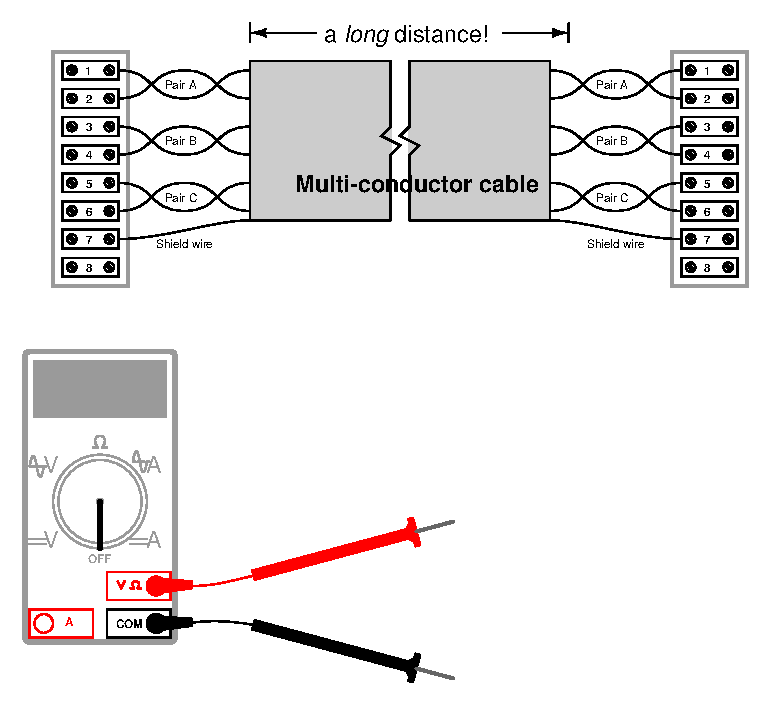
\includegraphics[width=15.5cm]{i00734x01.eps}$$

Faults you are looking for include {\it open} conductors, as well as {\it shorts} between conductors and/or shorts to ground.  Devise a series of tests you could perform with nothing but a multimeter to comprehensively check the electrical integrity of this cable.

\vfil 

\underbar{file i00734}
\eject
%(END_QUESTION)





%(BEGIN_ANSWER)

This is a graded question -- no answers or hints given!

%(END_ANSWER)





%(BEGIN_NOTES)

The fact that the cable is very long means the multimeter's test leads will not reach that far, and so we must find a creative way to test for continuity at just one end of the cable.  One such way is to connect all six signal conductors at one end of the cable, and then check for continuity (low resistance) between conductor pairs to check for the presence of open faults: 1-2, 1-3, 1-4, 1-5, 1-6, 2-3, 2-4, 2-5, 2-6, 3-4, 3-5, 3-6, 4-5, 4-6, 5-6.  If we measure no continuity (high resistance) between wires that are supposed to be connected, we know we have detected an open fault.

Without shorting the wires together at the far end of the cable, it is impossible to check for open faults.  In order to detect an open fault, you must first build a circuit where continuity is expected, and then test for a lack of continuity.  

\vskip 10pt

Checking for shorts does not require the wires to be joined.  In fact, we must separate all the cable's conductors in order to try to ensure no continuity between them, then we use the meter to check for continuity between any of those conductors and earth ground.  If we measure continuity between wires that are supposed to be separated, we know we have detected a shorted fault.

%INDEX% Electronics review: continuity-checking a multi-pair cable

%(END_NOTES)


